\chapter{Introdução}

Arquiterura de software de um programa é a estrutura que define as propriedades
externamente visíveis e o relacionamento entre os grandes componentes
estruturais do sistema \cite{engenhariaDeSoftwarePressman}, esta arquitetura
pode estar ou não documentada em forma de diagramas, grafos, tabelas e etc.
Todo projeto de software possui uma arquitetura implícita, ter esta arquitetura
documentada pode ser útil para possibilitar, por exemplo, a extração de
métricas de modularidade ou para estudar o impacto de possíveis alterações de
um projeto \cite{mata26-terceiro-projeto-piloto}.

Existem, hoje, diversas ferramentas capazes de extrair do código fonte ou do
código objeto a arquitetura de software de um sistema, entre as opções
pesquisadas \cite{sourceVersusObjectCodeExtraction} a maioria delas faz uso do
código objeto, ou seja, faz uso de dados resultantes da compilação do código
fonte.

Uma desvantagem em se utilizar código objeto é que fica impossível
analisar projetos que não compilem mais, seja por falhas no código ou por
possuir dependencias não satisfeitas. Além disso algumas informações como por
exemplo macros em projetos C/C++ são perdidas durante a
compilação \cite{sourceVersusObjectCodeExtraction}.

Este trabalho baseia-se na implementação de uma extensão para o egypt que
possibilite a extração de informação de dependências entre módulos de programas
C/C++ baseada em código fonte. O egypt é uma ferramenta originalmente escrita
com o objetivo de gerar gráficos de chamada entre funções de programas escritos
em C e que usa como base código objeto, ele será visto com mais detalhes na
seção~\ref{sec:egypt} do capítulo~\ref{ch:implementacao}.

Essa extensão para o egypt além de possibilitar analisar projetos que não
compilem mais trará informações mais precisas já que alguns dados importantes
não se perderão como acontece por exemplo com macros em projetos C/C++
\cite{sourceVersusObjectCodeExtraction} que se perdem com o extrator baseado em
GCC\sigla{GCC}{GNU C Compiler}.

Este trabalho está organizado da seguinte forma. No capítulo~\ref{ch:conceitos}
são abordados conceitos básicos de arquitetura de software e atributos de
modularidade como acoplamento e coesão. No capítulo~\ref{ch:implementacao} será
demonstrado como a ferramenta foi implementada. No capítulo~\ref{ch:avaliacao}
os resultados obtidos pela ferramenta são avaliados com um estudo de caso. O
capítulo~\ref{ch:conclusao} apresenta as conclusões e trabalhos futuros.

% ----------- CONCEITOS -------------

\chapter{Conceitos} \label{ch:conceitos}

Neste capítulo serão apresentados os conceitos fundamentais utilizados neste
trabalho para a avaliação dos resultados gerados pela ferramenta desenvolvida.

\section{Arquitetura de Software}

Arquitetura de software de um programa é a estrutura que define as propriedades
externamente visíveis e o relacionamento entre os grandes componentes
estruturais do sistema \cite{engenhariaDeSoftwarePressman}.

\citeonline{engenhariaDeSoftwarePressman} destaca 3 razões principais sobre a
importância da arquitetura de software:

\begin{itemize}
\item Representações da arquitetura de software constituem um facilitador da
comunicação entre todas as partes interessadas no desenvolvimento de um
sistema.
\item A arquitetura destaca decisões iniciais de projeto que terão um impacto
profundo em todo o trabalho de engenharia de software que se segue.
\item A arquitetura compõe uma representação de simples entendimento de como o
sistema é estruturado e como se interrelacionam os seus componentes.
\end{itemize}

Apesar de Pressman, aqui, destacar apenas a importancia da arquitetura de
software nas decisões iniciais do projeto, ela é de suma importancia durante
todo o processo de desenvolvimento de um projeto.

A arquitetura de grandes projetos de software raramente são documentados e
quando são usualmente estão desatualizados
\cite{sourceVersusObjectCodeExtraction}, ter a arquitetura documentada e
atualizada é importante, por exemplo, como forma apoio para os desenvolvedores e novos
colaboradores.

Neste trabalho a extração da arquitetura de software de um programa será
utilizada para cálculo de métricas que possibilitem avaliar a qualidade do
sistema em relação aos seus atributos de modularidade.

\section{Atributos de Modularidade}

A medição é um elemento fundamental para qualquer processo de engenharia
\cite{engenhariaDeSoftwarePressman}. As métricas de software são um modo
poderoso de prover indicadores de modularidade da arquitetura de um sistema
\cite{OntheModular}.

%Um dos conjuntos de métricas de software OO mais amplamente referenciado foi
Um dos conjuntos de métricas de software mais amplamente referenciado foi
proposto por Chidamber e Kemerer \cite{engenhariaDeSoftwarePressman}, eles
propuseram seis métricas:

\begin{description}
\item[WMC\sigla{WMC}{Weighted Methods per Class}] Métodos ponderados por classe (weighted methods per class).
\item[DIT\sigla{DIT}{Depth of the Inheritance Tree}] Profundidade de árvore de herança (depth of the inheritance tree).
\item[NOC\sigla{NOC}{Number of Children}] Número de filhos (number of children).
\item[CBO\sigla{CBO}{Coupling Between Objects classes}] Acoplamento entre as classes de objetos (coupling between objects classes).
\item[RFC\sigla{RFC}{Response For a Class}] Resposta de uma classe (response for a class).
\item[LCOM\sigla{LCOM}{Lack of Cohesion in Methods}] Falta de coesão em métodos (lack of cohesion in methods).
\end{description}

Este trabalho fundamenta-se em apenas 2 das métricas acima, CBO e LCOM, que são
métricas que levam em consideração atributos de acoplamento e coesão.

\subsection{Acoplamento}

Acoplamento é a medida qualitativa de conexões entre os componentes de um
sistema, ou simplesmente o número de colaborações entre as classes de um
determinado programa. Ele representa o nível de interdependências entre os
módulos de um sistema, quando maior o acoplamento maior a complexidade do
sistema.

É importante lembrar que apesar ser desejável baixo acoplamento o sistema deve
se comunicar interna e externamente, então o acoplamento é inevitável e em
alguns momentos não será possível diminuí-lo, nestes casos o importante é que
o projetista entenda as implicações disso.

A métrica para cálculo de acoplamento utilizada neste trabalho será CBO, esta
métrica é calculada contando-se o número de colaborações de uma classe com as
outras entidades do sistema. Na figura~\ref{fig:exemplo-cbo} a classe {\it
module1} tem CBO = 2.

\begin{figure}[h]
\center
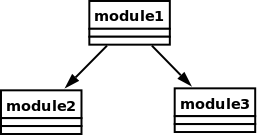
\includegraphics[scale=0.4]{imagens/exemplo-cbo}
\caption{Diagrama de classes exemplo para cálculo de CBO}
\label{fig:exemplo-cbo}
\end{figure}

Valores de CBO altos podem significar que a reusabilidade de uma classe é
pequena \cite{engenhariaDeSoftwarePressman}, além de implicar que a manutenção
e os testes serão mais complexos de serem feitos. Em geral o ideal é que os
valores de CBO sejam baixos.

\subsection{Coesão}

Coesão é e medida que define o quanto um módulo de um programa está focado em
solucionar um único problema. \citeonline{engenhariaDeSoftwarePressman} define
coesão da seguinte forma: ''{\it coesão} implica que um componente ou classe
encapsule somente os atributos e operações muito relacionados entre si e com a
classe ou componente propriamente dito''.

A métrica utilizada neste trabalho será a {\bf Falta de coesão em métodos}
({\it lack of cohesion in methods} - LCOM). LCOM é o número de métodos num
mesmo componente que compartilham os mesmos atributos, se nenhum método tem
acesso ao mesmo atributo então LCOM = 0. Na figura~\ref{fig:exemplo-lcom} a
classe {\it module1} tem LCOM = 2, onde a variável {\it nome} é compartilhada
entre os métodos {\it imprime} e {\it exporta}.

\begin{figure}[h]
\center
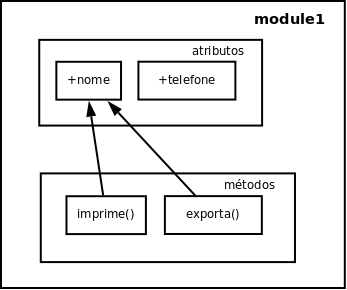
\includegraphics[scale=0.4]{imagens/exemplo-lcom}
\caption{Exemplo de troca de mensagens internas de module1 para cálculo de LCOM}
\label{fig:exemplo-lcom}
\end{figure}

É desejável que a coesão dos componentes de um sistema seja alta, isto garante
que o acoplamento do sistema seja baixo e como consequência a complexidade do
sistema cai facilitando a manutenção e o desenvolvimento. LCOM mede a falta de
coesão então valores baixos significam boa coesão, se LCOM é alto métodos podem
estar acoplados uns aos outros através de atributos, isto aumenta a
complexidade do projeto da classe.

A falta de coesão pode indicar que é melhor dividir a classe em subclasses
\cite{observationsOnLCOM}.

Após a definicial inicial de Chidamber e Kemerer para o cálculo de LCOM vários
autores propuseram modificações deste método, as mais significantes incluindo a
definição original são \cite{analysisOfLCOM}:

\begin{itemize}
\item A definição original por Chidamber e Kemerer - LCOM1;
\item A definição de Li e Henry - LCOM?;
\item A re-definição do LCOM de Li e Henry por Hitz e Montazerri - LCOM4; e
\item A re-definição da definição original por Chidamber and Kemerer - LCOM?.
\end{itemize}

O que é LCOM1, LCOM4, quais limitações, qual é melhor?

A definição original por Chidamber e Kemerer comumente chamada de LCOM1 e a
redefinição por Hitz e Montazerri conhecida como LCOM4 serão as métricas
abordadas neste trabalho.

A definição original LCOM1 após sua publicação recebeu várias críticas,
primeiro para classes muito diferentes ela dá valor zero. Segundo Gupta
\cite{aCritiqueOfCohesion} LCOM1 não é um caminho válido para medir coesão de
classes. 

LCOM1 é calculado da seguinte forma:

Considere C1 uma classe com M1, M2, \ldots, Mn métodos e Ii o conjunto de
atributos (variábeis de instancia) de C1 sendo usado pelo método Mi. Para cada
método Mi de C1 deve existir um grupo de atributos Ii correspondente.

Então, LCOM = Número distinto de grupos formados pela intersecção dos 'n'
conjuntos.

% ----------- IMPLEMENTACAO -------------

\chapter{Implementação do Extrator} \label{ch:implementacao}

\section{egypt} \label{sec:egypt}

O egypt foi originalmente desenvolvido por Andreas
Gustafsson\footnote{http://www.gson.org/egypt} com o objetivo de gerar gráficos
de chamada entre funções de programas escritos em C, ele funciona lendo os
arquivos intermediários gerados pelo GCC e os
converte num gráfico de chamada no formato usado pelo
Graphviz\footnote{http://www.graphviz.org}, um programa para visualização de
gráficos.

O egypt é Software Livre e em Janeiro de 2009 começou a ser restruturado por
Antonio Terceiro o qual o tem mantido
em\footnote{http://github.com/terceiro/egypt}. As principais mudanças sofridas
pelo egypt deste então foram \cite{structuralComplexityEvolution}:

\begin{itemize}
\item Detecção de uso de variáveis, para identificar que função usa qual
variável.
\item Opção para agrupar chamada e uso de variaveis por módulo, com isto é
possível ter uma visão de dependência entre módulos.
\item Refatoração do script egypt em um design orientado a objetos, para
permitir diferentes módulos de extração e relatório.
\item Geração de relatório de métricas, como coesão e acoplamento por exemplo.
\end{itemize}

Segue abaixo como ficou estruturado o egypt após a refatoração:

\begin{description}
\item[egypt] Script principal
\item[Egypt::Extractor] Extrator baseado nos arquivos intermediários do GCC
\item[Egypt::Metrics] Gera relatório de métricas com os dados do Egypt::Model
\item[Egypt::Model] Armazena os dados obtidos pelo extrator
\item[Egypt::Output::DOT] Gera saída no formato do Graphviz com os dados de Egypt::Model
\end{description}

\begin{figure}[h]
\center
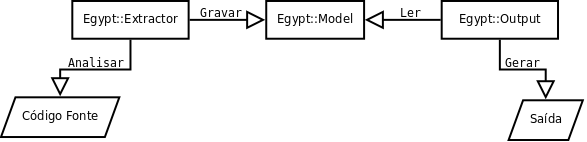
\includegraphics[scale=0.4]{imagens/egypt-fluxogram}
\caption{fluxograma de funcionamento do egypt}
\label{egypt-fluxogram}
\end{figure}

No fluxograma da figura~\ref{egypt-fluxogram} temos o seguinte: Egypt::Model é
alimentado com informações sobre declaração e uso de símbolos extraídos pelo
Egypt::Extractor e o Egypt::Output lê as informações contidas nele e gera saída
no formato apropriado.

\section{Doxygen (e a sua API)}

Doxygen\footnote{http://www.doxygen.org} é um sistema de documentação para C++,
C, Java, Objective-C, Python, IDL, Fortran, VHDL, PHP e C\#. Com ele é possível
gerar documentação em HTML, RTF, PostScript, PDF, \LaTeX\ e man pages, ele
extrai a documentação existente no código fonte e também extrai informações de
hierarquia e colaboração entre os módulos do projeto. É baseado nesta
capacidade de extrair informações de hierarquia e colaboração que o Doxygen foi
escolhido como base para implementação deste novo extrator para o egypt.

O Doxygen é Software Livre e está disponível sob a GPL\sigla{GPL}{GNU Public
License}v2 em
\footnote{https://doxygen.svn.sourceforge.net/svnroot/doxygen/trunk}, junto aos
fontes deste programa existe um pequeno exemplo chamado doxyapp, que foi usado
como base para este projeto já que ele implementa uma ferramenta para análise
de código fonte bem próximo as necessidades deste projeto.

Entre as inúmeras classes presentes na API\sigla{API}{Application Programming
Interface (ou Interface de Programação de Aplicativos)} do Doxygen é importante
destacar as seguintes:

\begin{description}
\item[Doxygen] Provê um namespace para varáveis e funções globais usadas pelo doxygen
\item[CodeOutputInterface] Interface de saída de trecho de código para os parsers
\item[MemberDef] Definição de um membro ou símbolo de classe
\item[FileDef] Definição de um arquivo
\end{description}


\section{Implementação do Extrator usando a API do Doxygen}

O Doxygen apesar de oferecer todos os recursos necessários para
analisar projetos C/C++ e extrair o uso de símbolos, como funções e variáveis,
que é o objetivo deste projeto, não possibilita que a saída gerada seja
customizada, apenas oferece opções específicas como PDF e HTML por exemplo. É
necessário então adaptar o Doxygen para gerar uma saída num formato
específico e apenas com as informações necessárias, para isto foi criado o
doxyparse, um parser capaz de analisar códigos C/C++ extraindo símbolos
com a identificação de onde são declarados e onde são utilizados.

Seguindo a interface CodeOutputInterface foi possível reaproveitar no doxyparse
todo o poder que o Doxygen fornece e gerar a saída da forma desejada. Na
figura~\ref{doxyparse-diagram} temos o diagrama desta implementação.

\begin{figure}[h]
\center
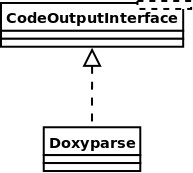
\includegraphics[scale=0.4]{imagens/doxyparse-diagram}
\caption{diagrama da hierarquia de classes do doxyparse}
\label{doxyparse-diagram}
\end{figure}

O doxyparse então reaproveita os recursos existentes no Doxygen para fazer a
análise de código e gerar uma saída que será lida pelo extrator a ser
implementado no egypt, ele redefine algums parâmetros de configuração
do Doxygen para obter o comportamento desejado, como: analisar diretórios
recursivamente, não gerar saida em Latex ou HTML, extrair tanta informação
quanto possível do código fonte, extrair informação de chamada e não gerar
mensagens de aviso.

O doxyparse faz então a análise dos fontes de um diretorio ou arquivo(s)
passados como parâmetro via linha de comando e extrai destes fontes os símbolos
encontrados. Após isto é gerada uma saída num formato específico que será lida
pelo extrator no egypt. Na figura~\ref{exemplo-saida-doxyparse} tem um exemplo
desta saída.

\begin{figure}[h]
\begin{Verbatim}[frame=single,fontsize=\relsize{-2},fontfamily=courier]
module module1.c
   function main in line 5
      uses function callback defined in module3.c
      uses function say_bye defined in module2.c
      uses function say_hello defined in module2.c
      uses variable variable defined in module3.c
\end{Verbatim}
\caption{exemplo de saída do doxyparse}
\label{exemplo-saida-doxyparse}
\end{figure}

Com a saída gerada pelo doxyparse o egypt precisa agora de um extrator que
entenda estes dados, extraia as informações sobre os símbolos e gere a saída no
formato do Graphviz que irá então gerar o gráfico de chamada entre os módulos.

O extrator atual do egypt, Egypt::Extractor, entende apenas arquivos
intermediários gerados pelo GCC e não é capaz de entender a saída da
figura~\ref{exemplo-saida-doxyparse}. Para isto foi necessário refatorar a
atual implementação do egypt e implementar um novo extrator. Na
figura~\ref{egypt-diagram-extractor} está o desenho desta nova estrutura.

\begin{figure}[h]
\center
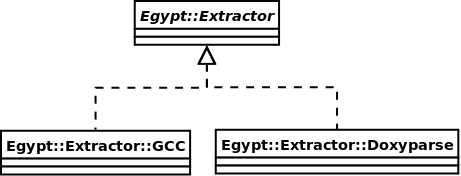
\includegraphics[scale=0.4]{imagens/egypt-diagram-extractor}
\caption{diagrama da hierarquia de classes do extrator do egypt}
\label{egypt-diagram-extractor}
\end{figure}

Abaixo uma breve descrição de cada classe presente na
figura~\ref{egypt-diagram-extractor}:

\begin{description}
\item[Egypt::Extractor] Interface padrão para os extratores.
\item[Egypt::Extractor::GCC] Extrator baseado nos arquivos intermediários do GCC.
\item[Egypt::Extractor::Doxyparse] Novo extrator baseado na saída do doxyparse
\end{description}

Após a refatoração demonstrada na figura~\ref{egypt-diagram-extractor} o egypt
pode extrair informações usando 2 métodos diferentes, usando o
Egypt::Extractor::GCC que faz a extração baseada nos arquivos intermediários do
GCC ou usando o Egypt::Extractor::Doxyparse que faz a análise utilizando o
doxyparse. Segue abaixo um exemplo de execução do egypt usando cada um dos
extratores:

\begin{Verbatim}[frame=single,fontsize=\relsize{-2},fontfamily=courier]
 $ egypt --extractor Doxyparse <arquivos>
 $ egypt --extractor GCC <arquivos>
\end{Verbatim}

% ----------- AVALIACAO -------------

\chapter{Avaliação} \label{ch:avaliacao}

Com o extrator pronto é necessário avaliar se as informações extraídas estão
corretas e se há diferenças em relação as informações extraídas pelo extrator
original do egypt baseado em GCC.

\section{Procedimento}

Em \cite{structuralComplexityEvolution} foi feita uma análise do
ristretto\footnote{http://goodies.xfce.org/projects/applications/ristretto}, um
Software Livre escrito em C para visualização de imagens no ambiente Desktop
Xfce\footnote{http://www.xfce.org}, utilizando o extrator original do egypt, as
informações geradas por esta análise serão utilizadas aqui para comparação com
as informações extraídas pelo novo extrator baseado no doxyparse.

Além da comparação entre o extrator original e o novo extrator a saída
gerada pelo doxyparse, o parser baseado no Doxygen, será analisada em
comparação com o código fonte em busca de inconsistências em relação a
declaração e uso de símbolos encontrados.

E por fim as métricas de coesão e acomplamento calculadas pelo egypt, usando
cada um dos dois extratores, serão analisadas com objetivo de identificar
possíveis diferenças entre cada um.

\section{Resultados}

O egypt foi executado utilizando o extrator Doxyparse e GCC em cada uma das versões
do ristretto, o egypt se comportou aparentemente de forma correta e extraiu sem problemas
e as informações esperadas.

Com os dados extraidos pelo Egypt::Extractor::GCC e Egypt::Extractor::Doxyparse
foram gerados gráficos de dependencia entre os módulos do projeto ristretto das
versões 0.0.1 até a 0.0.21.

O resultado dos 2 extratores não foi igual, na figura~\ref{ristretto-0.0.1}
temos o grafo gerado por cada extrator para o ristretto 0.0.1.

\begin{figure}
\center
\subfigure[Egypt::Extractor::Doxyparse]{
   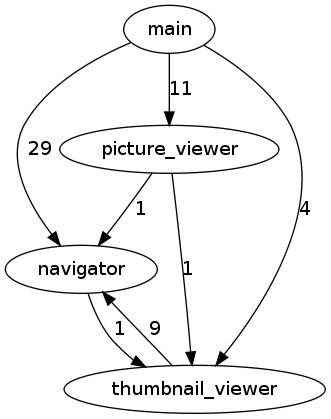
\includegraphics[scale=0.3]{imagens/ristretto-0_0_1-doxyparse}
   \label{ristretto-0.0.1-doxyparse}
}
\qquad
\subfigure[Egypt::Extractor::GCC]{
   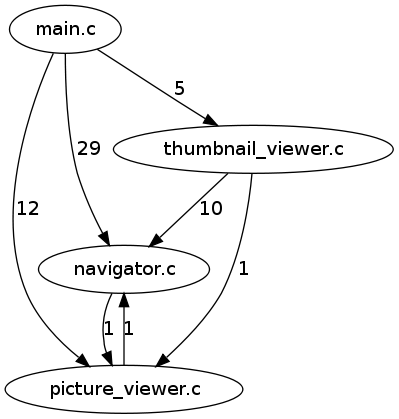
\includegraphics[scale=0.3]{imagens/ristretto-0_0_1-gcc}
   \label{ristretto-0.0.1-gcc}
}
\caption{gráfico de chamada entre módulos do {\bf Ristretto 0.0.1} gerado pelo Egypt}
\label{ristretto-0.0.1}
\end{figure}

Na figura~\ref{ristretto-0.0.1-gcc} por exemplo temos que o módulo {\it
navigator} chama {\it picture\_viewer}, e na
figura~\ref{ristretto-0.0.1-doxyparse} não temos esta chamada e sim que {\it
navigator} chama {\it thumbnail\_viewer}.

Na seção~\ref{sec:discussao} discutiremos os detalhes destas direferenças entre
cada extrator.

\section{Discussão} \label{sec:discussao}

Para comparação entre os dois extratores foram selecionadas 3 versões do
ristretto, a 0.0.1, 0.0.11 e 0.0.21, nas figuras \ref{ristretto-0.0.1},
\ref{ristretto-0.0.11} e \ref{ristretto-0.0.21} estão gráficos de chamadas
entre módulos de cada um. Algumas diferenças entre os gráficos
gerados pelo GCC e pelo Doxyparse foram notadas. 


Na figura~\ref{ristretto-0.0.1} nota-se uma diferença interessante entre as
informaçõe extraídas pelo GCC e o Doxyparse, há uma inversão entre os módulos
thumbnailer\_viewer e picture\_viewer. Enquanto o Doxyparse diz que o
picture\_viewer chama o thumbnailer\_viewer no GCC temos o contrário, após uma
verificação ao código fonte do ristretto 0.0.1 nota-se que nenhum dos 2 módulos
se referenciam, então os dois extratores estão dando informações incorretas.

O problema pode estar na interpretação dos dados pelo extrator ou nos dados
gerados pelo doxyparse. Ao investigar o problema foi possível notar que os
dados gerados pelo doxyparse estão corretos então o problema está no extrator. O
egypt armazena as informações usando como chave, ou seja, como identificador
único, o nome do símbolo em questão mas alguns módulos possuem símbolos com o
mesmo nome, isto faz com que o egypt confunda o uso e chamada destes símbolos.

A solução adotada para este problema foi armazenar o nome do módulo junto ao
nome do símbolo, por exemplo ao invés de guardar apenas parent\_class guarda-se
main::parent\_class. Na figura \ref{ristretto-0.0.1-doxyparse-2} temos o
gráfico atualizado após esta correcão.

\begin{figure}[h]
\center
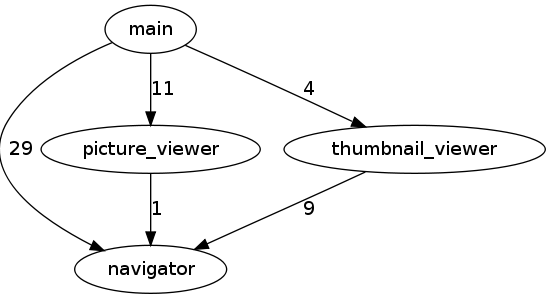
\includegraphics[scale=0.3]{imagens/ristretto-0_0_1-doxyparse-2}
\caption{gráfico de chamada entre módulos do {\bf Ristretto 0.0.1} gerado pelo Egypt::Extractor::Doxyparse atualizado}
\label{ristretto-0.0.1-doxyparse-2}
\end{figure}

\begin{figure}
\center
\subfigure[Egypt::Extractor::Doxyparse]{
   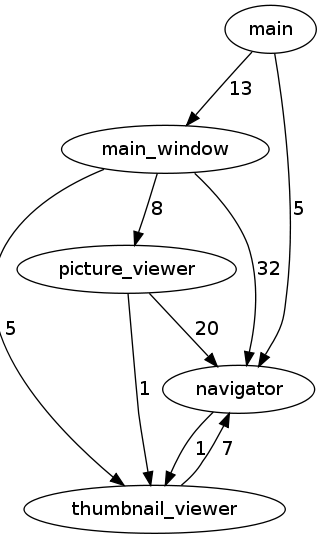
\includegraphics[scale=0.3]{imagens/ristretto-0_0_11-doxyparse}
   \label{ristretto-0.0.11-doxyparse}
}
\qquad
\subfigure[Egypt::Extractor::GCC]{
   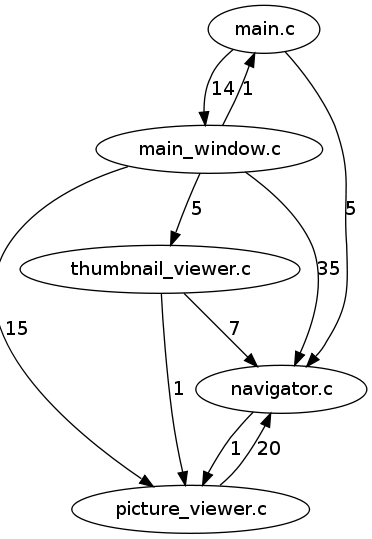
\includegraphics[scale=0.3]{imagens/ristretto-0_0_11-gcc}
   \label{ristretto-0.0.11-gcc}
}
\caption{gráfico de chamada entre módulos do {\bf Ristretto 0.0.11} gerado pelo Egypt}
\label{ristretto-0.0.11}
\end{figure}

Na figura~\ref{ristretto-0.0.11} o GCC diz que o módulo main\_window chama
main, já no Doxyparse não há esta chamada. E de fato, analisando o código fonte
do ristretto 0.0.11 não foi encontrada nenhuma chamada de main\_window para
main, então o Doxyparse está correto neste caso. Mas ele confunde alguns
símbolos como na figura~\ref{ristretto-0.0.1}, veja na
figura~\ref{ristretto-0.0.11-doxyparse-2} o gráfico atualizado após a correção.

\begin{figure}
\center
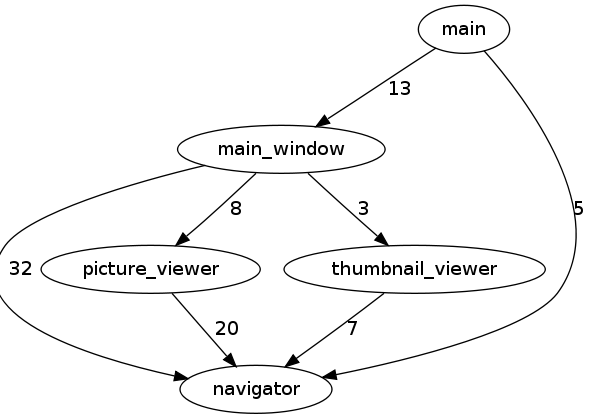
\includegraphics[scale=0.3]{imagens/ristretto-0_0_11-doxyparse-2}
\caption{gráfico de chamada entre módulos do {\bf Ristretto 0.0.11} gerado pelo Egypt::Extractor::Doxyparse atualizado}
\label{ristretto-0.0.11-doxyparse-2}
\end{figure}

Na figura~\ref{ristretto-0.0.21} temos outra diferença interessante, o GCC
informa que o módulo save\_dialog é chamado pelos módulos main\_window,
thumbnail, navigator, picture\_viewer e thumbnail\_bar sendo que no código
fonte do ristretto 0.0.21 não há indícios de que todos esses módulos chamem o
módulo save\_dialog, com excessão de main\_window. Já o Doxyparse dá uma
informação mais coerente onde apenas main\_window chama save\_dialog, mas o
Doxyparse dá uma informação controversa onde o save\_dialog chama
thumbnail\_bar e isto não foi confirmado analisando o código fonte do projeto.
Mas este problema foi causado pelo mesmo problema já corrigido nos exemplos
citados acima para as versões 0.0.1 e 0.0.11, veja na
figura~\ref{ristretto-0.0.21-doxyparse-2} o gráfico atualizado.

\begin{figure}
\center
\subfigure[Egypt::Extractor::Doxyparse]{
   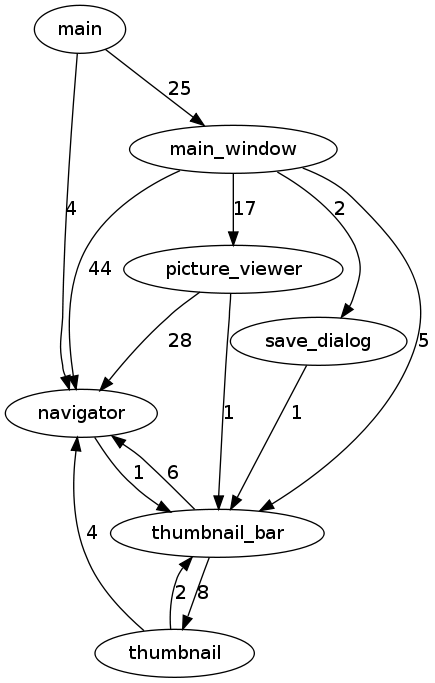
\includegraphics[scale=0.3]{imagens/ristretto-0_0_21-doxyparse}
   \label{ristretto-0.0.21-doxyparse}
}
\qquad
\subfigure[Egypt::Extractor::GCC]{
   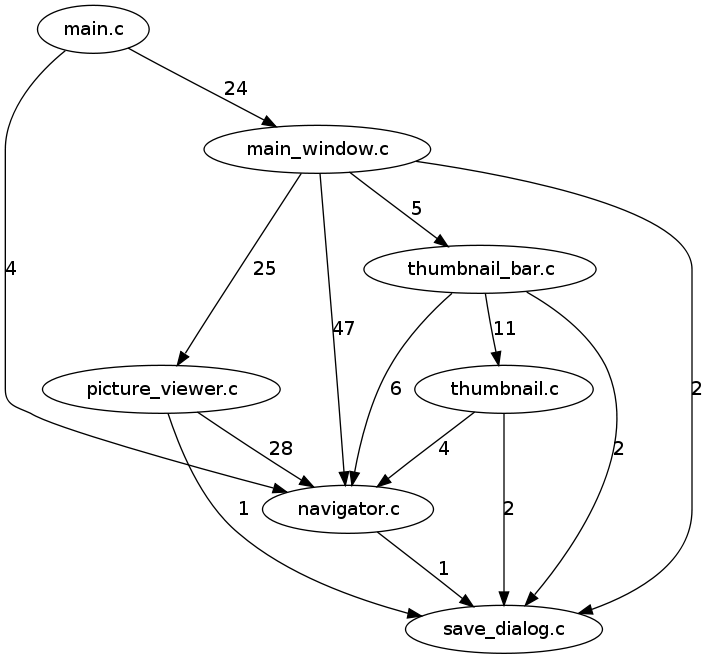
\includegraphics[scale=0.3]{imagens/ristretto-0_0_21-gcc}
   \label{ristretto-0.0.21-gcc}
}
\caption{gráfico de chamada entre módulos do {\bf Ristretto 0.0.21} gerado pelo Egypt}
\label{ristretto-0.0.21}
\end{figure}

Além destas correções no extrator foi necessário corrigir no doxyparse a
identificação dos símbolos estáticos, nesta avaliação feita com o ristretto o
doxyparse confunde o uso do simbolo parent\_class, uma variavei estática
definida por todos os módulos do projeto. O doxyparse registra a declaração
deste símbolo apenas na primeira vez que é encontrado e nas ocorrências de uso
e chamada nos diversos módulos o doxyparse faz referência ao primeiro módulo
onde o símbolo foi encontrado. Isto foi solucionado ignorando as chamadas aos
símbolos estáticos fora do módulo sendo analisado, ou seja, só se considera
chamada a símbolos estaticos se eles estiverem no mesmo módulo que o simbolo.

\begin{figure}
\center
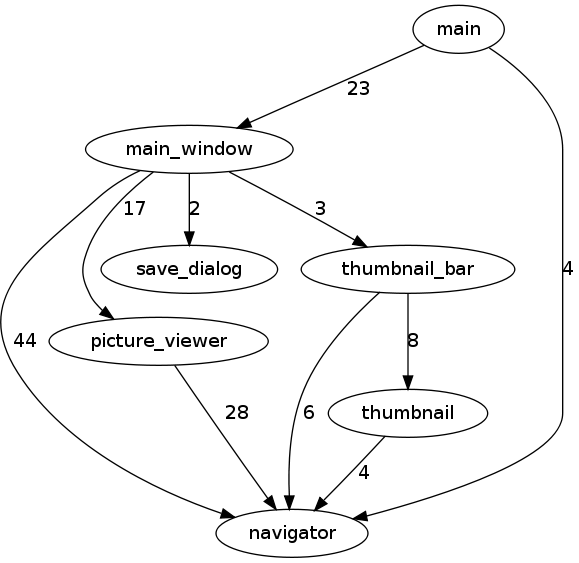
\includegraphics[scale=0.3]{imagens/ristretto-0_0_21-doxyparse-2}
\caption{gráfico de chamada entre módulos do {\bf Ristretto 0.0.21} gerado pelo Egypt::Extractor::Doxyparse atualizado}
\label{ristretto-0.0.21-doxyparse-2}
\end{figure}

Após a análise e interpretação das diferenças básicas encontradas entre o
Doxyparse e GCC iremos comparar os 2 em nível de métricas e as diferenças
encontradas e iremos interpretar essas diferenças encontradas.

Na tabela~\ref{tab:comparacao-metricas} temos resumo comparativo entre as
métricas calculadas pelo egypt, através de Egypt::Metrics, usando os extratores
GCC e Doxyparse em cada versão do ristretto. Onde é apresentado a média de
acoplamento e falta de coesão para cada versão. A métrica utilizada aqui em em
todo este trabalho para falta de coesão é a LCOM4.

\begin{table}
\caption{Métricas calculadas usando os extratores GCC e Doxyparse}
\centering
\begin{tabular}{| l | c c | c c |}
\hline
Extrator  & \multicolumn{2}{|c|}{GCC}        & \multicolumn{2}{|c|}{Doxyparse} \\
\hline
Média     & Falta de Coesão & Acoplamento    & Falta de Coesão & Acoplamento   \\
\hline
0.0.1     & 4.75            & 2.75           & 5.00            & 1.25          \\
0.0.2     & 5.75            & 2.75           & 6.00            & 1.25          \\
0.0.3     & 6.00            & 2.75           & 6.00            & 1.25          \\
0.0.4     & 6.25            & 2.75           & 6.25            & 1.25          \\
0.0.5     & 6.25            & 2.75           & 6.25            & 1.25          \\
0.0.6     & 7.60            & 3.00           & 7.60            & 1.40          \\
0.0.7     & 7.60            & 3.00           & 7.60            & 1.40          \\
0.0.8     & 7.00            & 3.00           & 7.20            & 1.40          \\
0.0.9     & 7.20            & 3.00           & 7.40            & 1.40          \\
0.0.10    & 7.60            & 3.00           & 8.00            & 1.40          \\
0.0.11    & 7.60            & 3.00           & 8.00            & 1.40          \\
0.0.12    & 7.60            & 3.00           & 8.00            & 1.40          \\
0.0.13    & 7.80            & 3.00           & 8.20            & 1.40          \\
0.0.14    & 8.00            & 3.00           & 8.40            & 1.40          \\
0.0.15    & 8.00            & 3.00           & 8.80            & 1.40          \\
0.0.16    & 7.16            & 3.16           & 7.83            & 1.50          \\
0.0.17    & 7.00            & 3.16           & 7.83            & 1.50          \\
0.0.18    & 7.50            & 3.00           & 8.33            & 1.50          \\
0.0.19    & 7.83            & 3.00           & 8.66            & 1.50          \\
0.0.20    & 8.83            & 3.00           & 10.00           & 1.50          \\
0.0.21    & 8.28            & 3.00           & 9.14            & 1.42          \\
\hline
\end{tabular}
\label{tab:comparacao-metricas}
\end{table}

Analisando a tabela é possível notar que o acoplamento calculado pelo Doxyparse
se mantém menor do que o GCC em todas as versões do ristretto, já a métrica de
Falta de Coesão LCOM4 se mantém ligeiramente maior também em todas as versões,
embora a diferença entre o Doxyparse e GCC seja pequena neste caso.

Qual será a causa destas diferenças? Vamos tentar explicar! Vamos analisar os
dados de cada módulo do ristretto 0.0.1. Na
tabela~\ref{tab:comparacao-metricas-ristretto-0.0.1} a métrica utilizada na
coluna falda de coesão é LCOM4.

\begin{table}
\caption{Métricas usando os extratores GCC e Doxyparse para o ristretto 0.0.1}
\centering
\begin{tabular}{| l | c c | c c |}
\hline
Extrator          & \multicolumn{2}{|c|}{GCC}        & \multicolumn{2}{|c|}{Doxyparse} \\
\hline
                  & Falta de Coesão & Acoplamento    & Falta de Coesão & Acoplamento   \\
\hline
main              & 1               & 4              & 1               & 3             \\
navigator         & 13              & 2              & 14              & 0             \\
picture\_viewer   & 2               & 2              & 2               & 1             \\
thumbnail\_viewer & 3               & 3              & 3               & 1             \\
\hline
\end{tabular}
\label{tab:comparacao-metricas-ristretto-0.0.1}
\end{table}

A diferença entre o acoplamento do módulo {\it navigator} é claramente
verificado pela figura~\ref{ristretto-0.0.1-doxyparse-2} onde verifica-se que
este módulo não chama nenhum outro módulo.

\chapter{Conclusão} \label{ch:conclusao}

Os resultados obtidos foram satisfatórios e atingiram o objetivo inicial que
foi possibilitar extração de dados sem necessidade de compilar o software em
questão, c\ldots

A conclusão eu devo escrever por último, deve conter algo assim: "Este trabalho
tinha objetivo tal e atingiu tal objetivo". Deve ter referencia de como foi
feito e se os resultados foram bons, medios, satisfatorios, ruins, etc. E ao
final deve ter trabalhos futuros que eu tenha interesse ou não de fazer.

Trabalhos futuros: verificar Natural Docs, semelhando ao Doxygen implementado
em Perl e suporta outras linguagens. Implementar no doxyparse detecção de chamada
indireta.
